\section{Joint shape matching}
\label{sec:matching}

Another fundamental problem in shape analysis is shape matching, which finds relations or maps between shapes. These maps allow us to transfer information across shapes and aggregate information from a collection of shapes for a better understanding of individual shapes (e.g., detecting shared structures such as skeletons or shape parts). \rev{They also provide a powerful platform for comparing shapes (i.e., with respect to different measures and at different places). As we can see from other sections, shape maps are widely applied in shape classification and shape exploration as well.}

So far, most existing research in shape matching has focused on matching pairs of shapes in isolation. We refer to~\cite{van-Kaick:2010:SSC} for a survey and to~\cite{Leordeanu:2005:SM,Lipman:2009:MVC,van-Kaick:2010:SSC,Ovsjanikov:2010:OPM,Kim:2011:BIM,Ovsjanikov:2012:FMF} for recent advances. Although significant progress has been made,
state-of-the-art techniques are limited to shapes that are similar to each other. \rev{On the other hand, these techniques tend to be insufficient among shape collections that possess large geometric and topological variations.}

The availability of large shape collections offers opportunities to address this issue. Intuitively, when matching two dissimilar shapes, we may utilize intermediate shapes to transfer maps. In other words, we can build maps between similar shapes, and use the composite maps to obtain maps between less similar shapes. As we will see shortly, this intuition can be generalized to enforcing a cycle-consistency constraint; namely composite maps along cycles should be the identity map and the composite map between any two shapes is path-independent.
%
In this section, we discuss joint shape matching techniques that take a shape collection and noisy maps as input, and output improved maps across the shape collection.
%In a broader picture, the problem of joint matching is related to a wide range of topics, including fusing partially overlapped range scans~\cite{Huber:2002:Thesis}, re-assembling fractured objects~\cite{Huang:2006:RFO}, solving jigsaw puzzles~\cite{Goldberg:2004:GAA,Cho:2010:JPS}, and DNA/RNA sequencing and modeling~\cite{Marande:2007:DNA}. In the following, we focus on the contributions most related to 3D shapes.

\subsection{Model graph and cycle-consistency}

To formulate the joint matching problem, we consider a model graph $\set{G} = (\set{S}, \mathcal{E})$ (c.f.~\cite{Huber:2002:Thesis}). The vertex set $\set{S} = \{S_1, \cdots, S_{n})\}$ consists of the input shapes. The edge set $\set{E}$ characterizes the pairs of shapes that are selected for performing pair-wise matching. For small-scale datasets, we typically match all pairs of shapes. For large-scale datasets, the edge set usually connects shapes that are similar according to a pre-defined shape descriptor~\cite{Kim:2012:FC,Huang:2013:FSL}, thus generating a sparse shape graph.

The key component of a joint matching algorithm is to utilize the so-called cycle-consistency constraint.  In particular, if all the maps in $\mathcal{G}$ are correct, then composite maps along any loops should be the identity map. This is true for maps that are represented as transformations (e.g., rotations and rigid/affine transformations), or full point-wise maps that can be described as permutation matrices). We can easily modify the constraint to handle partial maps; namely, each point, when transformed along a loop, either disappears or goes back to the original point (See \cite{Huang:2014:FMN} for details).

The cycle-consistency constraint is useful because the initial maps, which are computed between pairs of shapes in isolation, are not expected to satisfy the cycle consistency constraint. \rev{On the other hand, although we do not know which maps or correspondences are incorrect, we can detect inconsistent cycles.} These inconsistent cycles provide useful information for us to detect incorrect correspondences or maps, i.e., an inconsistent cycle indicates that at least one of the participating maps or correspondences is incorrect. To incorporate this observation into algorithms, one has to formulate the cycle-consistency constraint properly. Existing works in data-driven shape matching fall into two categories: combinatorial techniques and matrix recovery based techniques.  The reminder of this section provides the details.

\begin{figure}[t]
\centering
    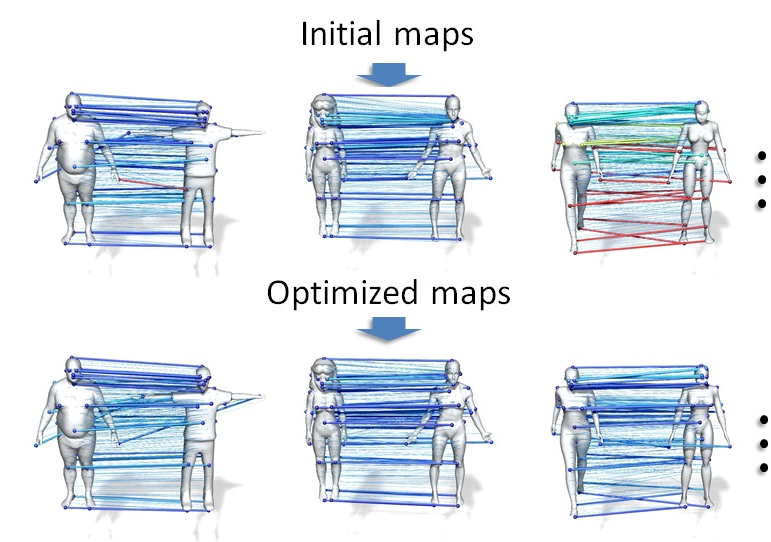
\includegraphics[width=1.0\columnwidth]{fig/img/huang_sig14_jsm.png}
    %\vspace{-0.4cm}
    \caption{Joint shape matching takes as input maps computed between pairs of shapes in isolation and utilizes the cycle-consistency constraint to improve shape maps. This figure shows the result of Huang et al.~\protect\cite{Huang:2014:FMN}, which performs joint shape matching under the functional map setting.}
    \label{fig:huang_sig14_jsm}
\end{figure}



\subsection{Combinatorial techniques}

\para{Spanning tree optimization.} Earlier works in joint matching aim at finding a spanning tree in the model graph. In~\cite{Goldberg:2004:GAA,Huang:2006:RFO}, the authors propose to use the maximum spanning tree (MST) of the model graph. However, this strategy can easily fail since a single incorrect edge in the MST may break the entire matching result. In the seminal work~\cite{Huber:2002:Thesis}, Huber showed that finding the best spanning tree maximizing the number of consistent edges is NP-hard. Although finding the best spanning tree is not tractable, Huber introduced several local operations for improving the score of spanning trees. \rev{However, these approaches are generally limited to small-scale problems so that the search space can be sufficiently explored.}

\para{Inconsistent cycle detection.} Another line of approaches~\cite{Zach:2010:DVR,Roberts:2011:SFM,Nguyen:2011:CSM} applies global optimization to select cycle-consistent maps. These approaches are typically formulated as solving constrained optimization problems, where objective functions encode the scores of selected maps, and constraints enforce the consistency of selected maps along cycles. The major advantage of these approaches is that the correct maps are determined globally. However, as the cycle consistency constraint needs to apportion blame along many edges on a cycle, the success of these approaches relies on the assumption that correct maps are dominant in the model graph so that the small number of bad maps can be identified through their participation in many bad cycles.

\para{MRF formulation.} Joint matching may also be formulated as solving a second order Markov Random Field (or MRF)~
\cite{Cho:2010:JPS,Cho:2010:TPT,Crandall:2011:DOL,Huang:2012:OAE}. The basic idea is to sample the transformation/deformation space of each shape to obtain a candidate set of transformation/deformation samples per shape. Joint matching is then formulated as optimizing the best sample for each shape. The objective function considers initial maps. Specifically, each pair of samples from two different shapes would generate a candidate map between them. The objective function then formulates second-order potentials, where each term characterize the alignment score between these candidate maps and the initial maps~\cite{Huang:2013:FSL,Huang:2012:OAE}.

The key challenge in the MRF formulation is generating the candidate samples for each shape. The most popular strategy is to perform uniform sampling~\cite{Crandall:2011:DOL,Huang:2013:FSL}, which works well when the transformation space is low-dimensional. To apply the MRF formulation on high-dimensional problems, Huang et al.~\cite{Huang:2012:OAE} introduce a diffusion-and-sharpening strategy. The idea is to diffuse the maps among the model graph to obtain rich samples of candidate transformations or correspondences and then perform clustering to reduce the number of candidate samples.


\subsection{Matrix based techniques}



A recent trend in map computation is to formulate joint map computation as inferring matrices~\cite{Singer:2011:VDM,Huang:2012:OAE,Kim:2012:FC,Huang:2013:SDP,journals/corr/abs-1211-2441,Chen:2014:SDP,Huang:2014:FMN}. The basic idea is to consider a big map collection matrix
$$
\vec{X} = \left [
\begin{array}{cccc}
\vec{X}_{11} & \vec{X}_{12} & \cdots & \vec{X}_{1n} \\
\vec{X}_{21} & \vec{X}_{22} & \cdots & \vec{X}_{2n} \\
\vdots & \ddots & \cdots & \vdots \\
\vec{X}_{21} & \cdots & \cdots & \vec{X}_{nn}
\end{array}
\right],
$$
where each block $\vec{X}_{ij}$ encodes the map from shape $S_i$ to shape $S_j$. In this matrix representation, the cycle-consistency constraint can be equivalently described by simple properties of $\vec{X}$, i.e., depending on the types of maps, $\vec{X}$ is either positive semidefinite or low-rank (c.f.~\cite{Huang:2013:SDP,Huang:2014:FMN}). In addition, we may view the initial pair-wise maps as noisy measurements of the entries of $\vec{X}$. Based on this perspective, we can formulate joint matching as matrix recovery from noisy measurements of its entries.

\para{Spectral techniques.} The initial attempts in matrix recovery are spectral techniques and their variants~\cite{Singer:2011:VDM,Kim:2012:FC,Wang:2013:FMap}. The basic idea is to consider the map collection $\vec{X}^{\textup{input}}$ that encodes initial maps in its blocks. Then, the recovered matrix is given by $\vec{X} = \vec{U}\Sigma \vec{V}^{T}$, where $\vec{U}, \Sigma, \vec{V}$ represent the singular value decomposition (or SVD) of $\vec{X}^{\textup{input}}$. Various methods have added heuristics on top of this basic procedure. For example, Kim et al.~\cite{Kim:2012:FC} use the optimized maps to recompute initial maps.

This SVD strategy can be viewed as matrix recovery because $\vec{X}$ is equivalent to the optimal low-rank approximation of $\vec{X}^{\textup{input}}$ (with given rank) under the matrix Frobenius norm. However, as the input maps may contain outliers, employing the Frobenius norm for matrix recovery is sub-optimal. Moreover, it is hard to analyze these techniques, even in the very basic setting where maps are given by permutation matrices~\cite{conf/nips/PachauriKS13}.


\begin{figure}[t!]
\centering
    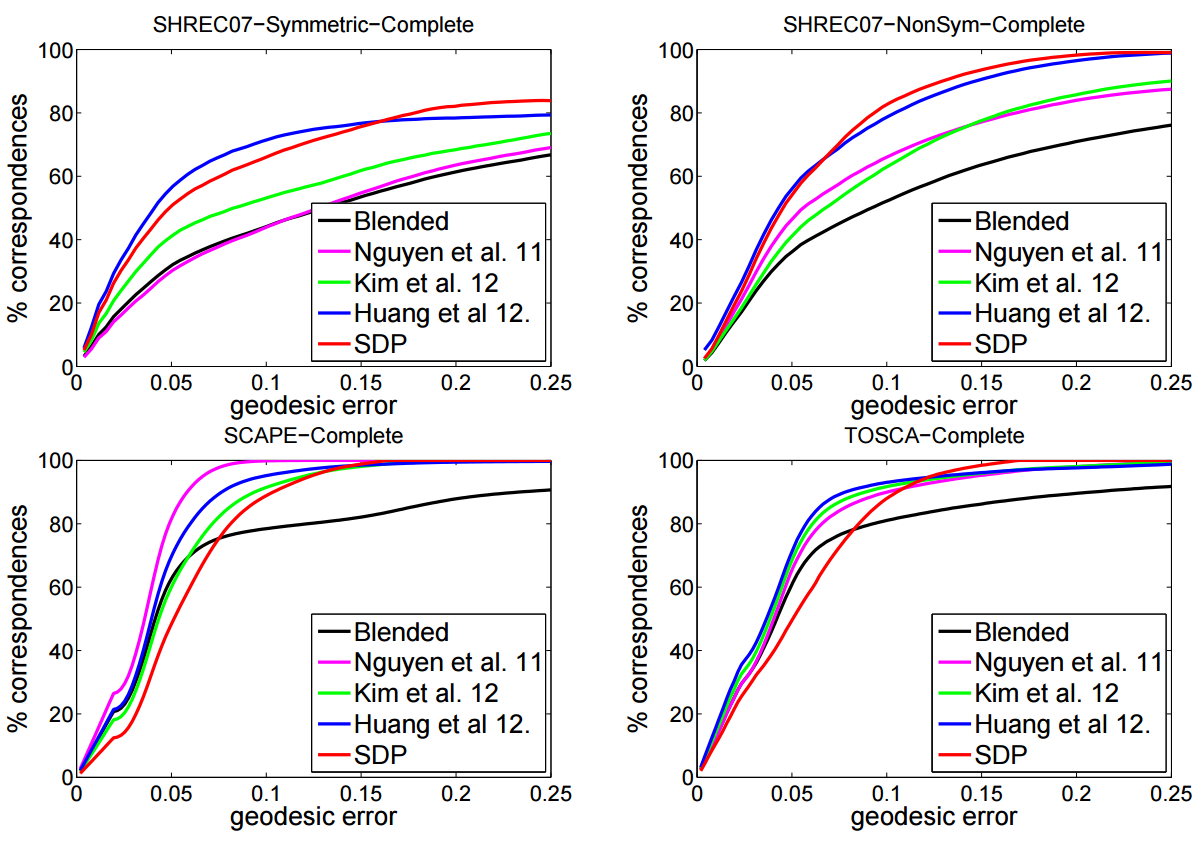
\includegraphics[width=1.0\columnwidth]{fig/img/map_evaluation.png}
    \vspace{-.5cm}
    \caption{\rev{Comparison among various data-driven shape matching methods: optimized composite maps~\protect\cite{Nguyen:2011:CSM}, fuzzy correspondences~\protect\cite{Kim:2012:FC},
hub-and-spoke network~\protect\cite{Huang:2012:OAE} and semidefinite programming relaxation~\protect\cite{Huang:2013:SDP}. The input maps are given by blended
intrinsic maps~\protect\cite{Kim:2011:BIM}.}}
    \label{fig:map_evaluation}
\end{figure}

\para{Point-based maps.} In a series of works, Huang and coworkers~\cite{Huang:2013:SDP,Chen:2014:SDP,cg-ssrmrf-14} consider the case of point-based maps and develop joint matching algorithms that admit theoretical guarantees. The work of~\cite{Huang:2013:SDP} considers the basic setting of permutation matrix maps and proves the equivalence between cycle-consistent maps and the low-rank or positive semi-definiteness of the map collection matrix. This leads to a semidefinite programming formulation for joint matching. In particular, the L1 norm is used to measure the distance between the recovered maps and the initial maps. The authors provide exact recovery conditions, which state that the ground-truth maps can be recovered if the percentage of incorrect correspondences in the input maps is below a constant. \rev{In a followup work, Chen et al.~\cite{Chen:2014:SDP} extends this to partial maps and provide a better analysis in the case where incorrect correspondences in the input maps are random.} The computational issue is addressed in~\cite{cg-ssrmrf-14}, which employs the alternating direction of multiplier methods for optimization. Figure~\ref{fig:map_evaluation} compares the SDP formulation of~\cite{Huang:2013:SDP} with several other data-driven shape matching methods. Note that all data-driven shape matching methods improve upon pair-wise matching, yet the SDP formulation leads to the largest improvement.

\para{Rotations and functional maps.} Maps that are represented by general matrices (e.g., rotations or functional maps) can also be handled in a similar fashion. In~\cite{journals/corr/abs-1211-2441}, Wang and Singer consider the case of rotations between objects. Their formulation is similar to~\cite{Huang:2013:SDP} but utilize an L1 Frobenius norm for measuring the distance between initial rotations and recovered rotations. Recently, Huang et al.~\cite{Huang:2014:FMN} extend this idea to functional maps. The major difference between functional maps and point-based maps or rotations is that the map collection matrix is no-longer symmetric. Thus, their method is formulated to recover low-rank matrices.


\subsection{Discussion and future directions}

The key to joint shape matching is to have a proper formulation of the cycle-consistency constraint. We have witnessed the evolution of this constraint from earlier works on combinatorial search and inconsistent cycle detection to more recent works which use spectral techniques, MRF based methods and matrix recovery techniques. In particular, matrix recovery techniques admit theoretical guarantees, providing a fundamental understanding of why joint shape matching can improve upon isolated pair-wise matching.

One future direction is to integrate pair-wise matching and joint matching into one optimization problem. Since the major role of joint matching is to remove the noise presented in pair-wise matching, it makes sense to perform them together. Such unified approaches have the potential to further improve upon decomposed approaches (i.e., from pair-wise to joint). The technical challenge is to find map representations so that pair-wise matching and map consistency can be formulated in the same framework.

%As we will discuss later, one of applications of map computation is in organizing big geometric data. Thus, it is important to develop data-driven matching techniques that are scalable to big geometric data. None of existing data-driven shape matching techniques can handle shape collections with more than thousands of shapes. In a recent paper, Huang et al.~\cite{Huang:2014:FMN} introduce a multi-layer map computation framework so that map computation may be distributed. The method essentially divide the input data into clusters and perform joint map computation among each cluster independently. The next layer builds maps between clusters. Maps between shapes are composed from maps with clusters and cluster-maps.  Still, there are plenty of open questions left including how to build the hierarchical map structure and what is the fundamental difference between a multi-layer structure and a single-layer structure (e.g., the techniques described above).
